\section{Introduction}
The original model from NASIC calculates a single endurance or range of an aircraft depending on inputs from a user. This method is deemed $\pm 5\%$ accurate based on comparing the output to explicit mission runs from a production program. With the tradeoff frontier of the developed methodology, a series of these outputs can be estimated with given flight parameters of the aircraft. To show the differences between the estimated frontier and the original model, several data points were extracted for three different aircraft, with the last aircraft having four differing configurations depending on external fuel and payload. This resulted in six tests for the developed methodology.\par
\section{Analysis Aircraft Parameters}
From an individual output from the original model, the parameters of the aircraft are derived based on the averages at specific altitudes and weights as discussed in Section \ref{section:modelUsage}. The following table describes all the parameters for each of the six aircraft used.
\begin{table}[H]
\caption{Aircraft Parameters}
\label{tab: aircraft parameters}
\resizebox{\textwidth}{!}{%
\begin{tabular}{|l|c|c|c|c|c|c|}
\hline
                             & \textbf{F-15C} & \textbf{F-16C} & \textbf{AC1-000} & \textbf{AC2-000} & \textbf{AC3-000} & \textbf{AC4-000} \\ \hline
\textbf{TSFC}                & 1.159    & 1.206    & 1.303       & 1.232      & 1.209      & 1.180      \\ \hline
\textbf{$C_L/C_D$}                 & 8.520           & 9.880           & 9.447     & 7.930            & 7.655            & 7.860             \\ \hline
\textbf{Mach}                & 0.732         & 0.791        & 0.865     & 0.830           & 0.808        & 0.759           \\ \hline
\textbf{Fuel To Cruise}      & 42738          & 26474          & 24006            & 25471            & 27780            & 33809            \\ \hline
\textbf{Distance To Cruise}  & 31.28          & 24.84          & 28.635           & 37.605           & 44.045           & 61.64            \\ \hline
\textbf{Combat Fuel}         & 688            & 402            & 402              & 402              & 402              & 402              \\ \hline
\textbf{Climb Fuel}          & 523            & 177            & 208              & 204              & 215              & 247              \\ \hline
\textbf{Percent Reserve}     & 5              & 5              & 5                & 5                & 5                & 5                \\ \hline
\textbf{Minutes Reserve}     & 20             & 20             & 20               & 20               & 20               & 20               \\ \hline
\textbf{Egress Dry Weight}   & 31262          & 20305          & 18188            & 19797            & 20062            & 19500            \\ \hline
\textbf{Egress Full Weight}  & 44710          & 27470          & 25155            & 26764            & 29211            & 35616            \\ \hline
\textbf{Ingress Dry Weight}  & 30645          & 20107          & 17879            & 17879            & 17890            & 17748            \\ \hline
\textbf{Ingress Full Weight} & 44093          & 27272          & 24846            & 24846            & 24857            & 24715            \\ \hline
\textbf{Cruise Altitude}     & 30000          & 30000          & 30000            & 30000            & 30000            & 30000            \\ \hline
\textbf{Loiter Altitude}     & 30000          & 30000          & 30000            & 30000            & 30000            & 30000            \\ \hline
\end{tabular}
}
\end{table}
The cruise and loiter altitude describe the altitude at which these parameters were derived. These are then estimated for different altitudes using US Standard Atmosphere. The ACX-000 aircraft is a dataset for which the aircraft is unknown to test whether the method is agnostic to a particular aircraft.

\section{Aircraft Tradeoff Comparison}
The tradeoff frontier was compared to the NASIC model using point statistics. Between three and eight points were generated from the NASIC model depending on data availability of the aircraft. These points were generated at ten, twenty, and thirty minutes of endurance for all aircraft, but if an aircraft was able to endure longer, the points at 40, 60, 80, and 100 minutes of endurance may have also been generated. The difference statistics were computed as the average of the absolute value of the difference between the tradeoff frontier, $E$, and the NASIC model, $O$.
\begin{equation}
    D_{avg} = \dfrac{\sum_{i = 1}^n |O_i-E_i|}{n}
\end{equation}
where $n$ is the number of points generated for an aircraft and $D_{avg}$ is reported in minutes. In addition, the maximum difference between an expected value from the tradeoff frontier and the NASIC model were computed for each aircraft at each altitude which is a statistic of the model's variability over different endurances.
\begin{table}[H]
\caption{Difference Statistics Between NASIC Model and Tradeoff Model}
\label{tab:diffstatistics}
\resizebox{\textwidth}{!}{%
\begin{tabular}{|l|c|c|c|c|c|c|}
\hline
                                    & \textbf{F-15C} & \textbf{F-16C} & \textbf{AC1-000} & \textbf{AC2-000} & \textbf{AC3-000} & \textbf{AC4-000} \\ \hline
\textbf{$D_{avg}$ at 30,000ft}     & 3.537          & 5.385          & 2.614            & 4.775            & 2.778            & 22.742           \\ \hline
\textbf{Max Mins at 30,000ft} & 5.790          & 9.817          & 5.151            & 4.891            & 4.154            & 23.740           \\ \hline
\textbf{$D_{avg}$ at 20,000ft}     & 3.083          & 5.403          & 2.403            & 2.628            & 5.059            & 23.496           \\ \hline
\textbf{Max Mins at 20,000ft} & 5.686          & 9.506          & 4.174            & 3.362            & 5.334            & 24.055           \\ \hline
\textbf{$D_{avg}$ at 10,000ft}     & 4.622          & 4.838          & 3.460            & 3.001            & 4.566            & 21.146           \\ \hline
\textbf{Max Mins at 10,000ft} & 5.872          & 8.772          & 5.112            & 3.568            & 4.910            & 22.710           \\ \hline
\end{tabular}%
}
\end{table}
These statistics showed minimal differences between the NASIC model's points and the tradeoff frontier's generated solution in the first five aircraft. There is a larger deviation in the second aircraft, but the trend of the data is the same as the trend-line from the tradeoff frontier. The following figures show the six aircraft's tradeoff frontiers mapped with the observed data points from NASIC's model.
\begin{figure}%
    \centering
    \subfloat[Comparison at 30,000 ft]{{\includegraphics[width=5cm]{Thesis/Analysis/Tradeoff_Pics/30000f15.eps} }}%
    \qquad
    \subfloat[Comparison at 20,000 ft]{{\includegraphics[width=5cm]{Thesis/Analysis/Tradeoff_Pics/20000f15.eps} }}%
    \qquad
    \subfloat[Comparison at 10,000 ft]{{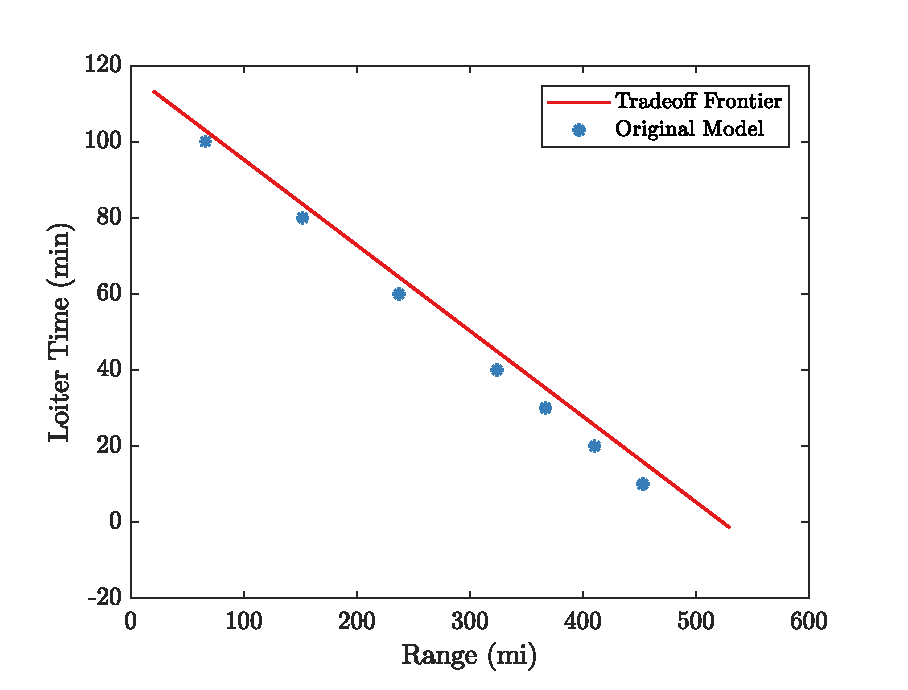
\includegraphics[width = 5cm]{Thesis/Analysis/Tradeoff_Pics/10000f15.eps} }}
    \caption{Tradeoff Comparison for F-15C}%
    \label{fig:tradef15}
\end{figure}

\begin{figure}%
    \centering
    \subfloat[Comparison at 30,000 ft]{{\includegraphics[width=5cm]{Thesis/Analysis/Tradeoff_Pics/30000f16.eps} }}%
    \qquad
    \subfloat[Comparison at 20,000 ft]{{\includegraphics[width=5cm]{Thesis/Analysis/Tradeoff_Pics/20000f16.eps} }}%
    \qquad
    \subfloat[Comparison at 10,000 ft]{{\includegraphics[width = 5cm]{Thesis/Analysis/Tradeoff_Pics/10000f16.eps} }}
    \caption{Tradeoff Comparison for F-16C}%
    \label{fig:tradef16}
\end{figure}

\begin{figure}%
    \centering
    \subfloat[Comparison at 30,000 ft]{{\includegraphics[width=7cm]{Thesis/Analysis/Tradeoff_Pics/30000c1.eps} }}%
    \qquad
    \subfloat[Comparison at 20,000 ft]{{\includegraphics[width=7cm]{Thesis/Analysis/Tradeoff_Pics/20000c1.eps} }}%
    \qquad
    \subfloat[Comparison at 10,000 ft]{{\includegraphics[width = 7cm]{Thesis/Analysis/Tradeoff_Pics/10000c1.eps} }}
    \caption{Tradeoff Comparison for AC1-000}%
    \label{fig:tradec1}
\end{figure}

\begin{figure}%
    \centering
    \subfloat[Comparison at 30,000 ft]{{\includegraphics[width=7cm]{Thesis/Analysis/Tradeoff_Pics/30000c2.eps} }}%
    \qquad
    \subfloat[Comparison at 20,000 ft]{{\includegraphics[width=7cm]{Thesis/Analysis/Tradeoff_Pics/20000c2.eps} }}%
    \qquad
    \subfloat[Comparison at 10,000 ft]{{\includegraphics[width = 7cm]{Thesis/Analysis/Tradeoff_Pics/10000c2.eps} }}
    \caption{Tradeoff Comparison for AC2-000}%
    \label{fig:tradec2}
\end{figure}

\begin{figure}%
    \centering
    \subfloat[Comparison at 30,000 ft]{{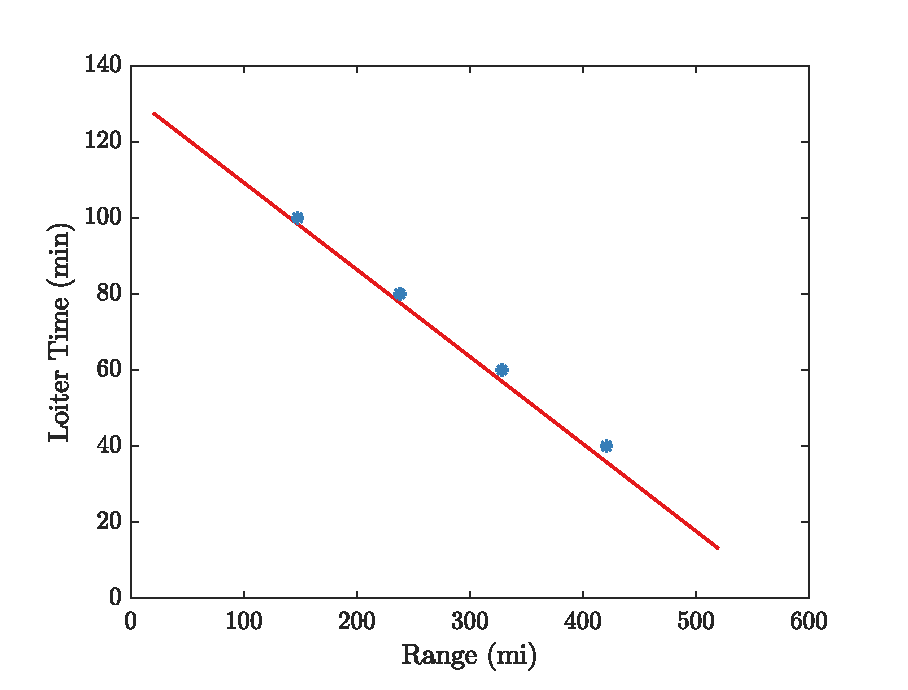
\includegraphics[width=7cm]{Thesis/Analysis/Tradeoff_Pics/30000c3.eps} }}%
    \qquad
    \subfloat[Comparison at 20,000 ft]{{\includegraphics[width=7cm]{Thesis/Analysis/Tradeoff_Pics/20000c3.eps} }}%
    \qquad
    \subfloat[Comparison at 10,000 ft]{{\includegraphics[width = 7cm]{Thesis/Analysis/Tradeoff_Pics/10000c3.eps} }}
    \caption{Tradeoff Comparison for AC3-000}%
    \label{fig:tradec3}
\end{figure}

\begin{figure}%
    \centering
    \subfloat[Comparison at 30,000 ft]{{\includegraphics[width=7cm]{Thesis/Analysis/Tradeoff_Pics/30000c4.eps} }}%
    \qquad
    \subfloat[Comparison at 20,000 ft]{{\includegraphics[width=7cm]{Thesis/Analysis/Tradeoff_Pics/20000c4.eps} }}%
    \qquad
    \subfloat[Comparison at 10,000 ft]{{\includegraphics[width = 7cm]{Thesis/Analysis/Tradeoff_Pics/10000c4.eps} }}
    \caption{Tradeoff Comparison for AC4-000}%
    \label{fig:tradec4}
\end{figure}
Overall, the tradeoff comparison relayed results on the same order of magnitude as the observed data points from NASIC's model. The maximum minutes that the model deviated from the observed points for the first two aircraft (for which the most test points were acquired) was by approximately ten minutes. This showed that the tradeoff frontier was consistent with results from the NASIC model and can sufficiently estimate the results at a high speed.\par
The final comparison of the four different configurations of ACX-000 displayed the main weakness in the analysis. Averaging the coefficient of lift over drag, thrust-specific fuel consumption, and speed of an airframe over the course of an aircraft's weight will effect the results when the difference between an outbound aircraft with a payload and external fuel tanks and the same inbound aircraft is large. The breakdown appears to happen in the comparison of AC4-000 where the aircraft is loaded with a large amount of external fuel. As a result, the estimation of the tradeoff frontier is conservative with the loiter time below the observed points by about twenty minutes on average. \par
With the tradeoff comparison similar to the results of the NASIC model, a loiter time comparison can be determined in seconds with the methodogy. AC1-000